\documentclass[12pt]{article}
\usepackage{amsmath}
\usepackage{bm}
\usepackage{graphicx}

\begin{document}

\pagebreak
\tableofcontents
\pagebreak

\section{Question 1}
We have an system of linear equations for which:
\begin{align}
x+y+z &= 2 \\
x + 4y - z &= k \\
2x-y + 4z &= k^2 
\end{align} 

We can throw it into an augmented matrix:
\begin{align*}
\left(\begin{array}{ccc|c}
1 & 1 & 1 & 2 \\
1 & 4 & -1 & k \\
2 & -1 & 4 & k^2
\end{array}\right)
\end{align*}
The row operations (which reduces it into row echelon form are as follows:
\begin{align}
\left(\begin{array}{ccc|c}
1 & 1 & 1 & 2 \\
0 & 3 & -2 & k-2 \\
0 & -3 & 2 & k^2-4
\end{array}\right)
\begin{array}{l}
  \text{$R_1$}\\
  \text{$R_2 \longmapsto R_2-R_1$}\\
  \text{$R_3 \longmapsto R_3-2R_1$ }
\end{array}
\\
\left(\begin{array}{ccc|c}
1 & 1 & 1 & 2 \\
0 & 3 & -2 & k-2 \\
0 & 0 & 0 & k^2+k-6
\end{array}\right)
\end{align}
The left side of the last row of the augmented matrix contains a row of zeros so we can solve for k:
\begin{align}
 k^2+k-6=0
\end{align}
If we solve equation $(6)$ for k we will get $\bm{k = -3}$ and $\bm{k=2}$.  \\
\newpage
\subsection{Cases Where There Are Infinite Amount of Solutions}

If we substitute  $k = -3$ and $k =2$ into the last row of $(5)$
will be $0x + 0y + 0z = 0$. Hence for  $k = -3$ and $k =2$, there will be {\bf infinite} amount of solutions to this system. The planes will meet in a infinite long line if $k = -3$ and $k =-2$.

To solve for the line we can make:
\begin{align}
z=t
\end{align}
and solve $R_2$ in $(5)$ for $y$ which is:
\begin{align*}
3y-2t=k-2
\end{align*}
Because $k$ has two possible values due to $R_2$ in (5), we will end up with 2 lines depending on the value of $k$ \\
\subsubsection{If $\bm{k=2}$}
Let $k = 2$:
\begin{align}
3y-2t&=0 \\
y&=\frac{2t}{3}
\end{align}
If we look back at $R_1$ of $(5)$ we get a equation of:
\begin{align}
x+y+z&=2
\end{align}
Substitute $(7)$ and $(9)$ into $(10)$ gives:
\begin{align}
x+\frac{5t}{3}&=2 \\
x&= 2 -\frac{5t}{3}
\end{align}
Therefore in the end our line when $k = 2$ will be:
\begin{align*}
x&=2-\frac{5t}{3} \\
y&=\frac{2t}{3} \\ 
z&=t
\end{align*}

\newpage

\subsubsection{If $\bm{k=-3}$}
Let $k = -3$:
\begin{align}
3y-2t&=-5 \\
y&=\frac{2t-5}{3}
\end{align}
If we look back at $R_1$ of $(5)$ again we get a equation of:
\begin{align*}
x+y+z&=2
\end{align*}
Substitute $(7)$ and $(14)$ into $(10)$ gives:
\begin{align}
x+\frac{2t-5}{3}+\frac{3t}{3}&=2 \\
x&= 2 -\frac{5t-5}{3}
\end{align}
Therefore in the end our line when $k = -3$ will be:
\begin{align*}
x&=2-\frac{5t-5}{3} \\
y&=\frac{2t-5}{3} \\ 
z&=t
\end{align*}


\subsection{Cases Where There Are No Solutions}
If $\bm{k \neq 2}$ or $\bm{k \neq -3}$ there will be {\bf no} solutions for this system as $0x + 0y + 0z \neq k^2+k-6$ when $k \neq 2$ or $k \neq -3$.

\subsection{Cases Where The Planes Meet At A Point}
It is not possible for this system to meet at one point because the left side of last row in $(5)$ is full of zeros. 

\newpage

\section{Question 2}
We want to prove that $\bm{A(B+C)=AB+AC}$.\\
Let's $\bm{A}$ to be a $\bm{m \times n}$ matrix and $\bm{B,C}$ to be a  $\bm{n \times p}$ matrix.
So $AB$ and $AC$ are both $\bm{m \times p}$ matrix. \\
Let $1 \leq i \leq m$ and $i \leq j \leq p$.\\
Let's consider the entry in $i$-th row and $j$-th column of $A(B+C)$.
\begin{align*}
[A(B+C)]_{ij}&=\sum^n_{k=1}(A)_{ik}(B+C)_{kj}\\
&=\sum^n_{k=1}(A)_{ik}\left[(B)_{kj}+(C)_{kj}\right]\\
&\text{Because We are manipulating real numbers here the following is allowed:}\\
&=\sum^n_{k=1}\left[(A)_{ik}(B)_{kj}+(A)_{ik}(C)_{kj}\right]\\
&=\sum^n_{k=1}(A)_{ik}(B)_{kj}+\sum^n_{k=1}(A)_{ik}(C)_{kj}\\
&\text{Using the definition of matrix multiplication we get:}\\
&=(AB)_{ij}+(AC)_{ij}\\
&=(AB+AC)_{ij}\\
&\text{The results above implies that:}\\
A(B+C)&=AB+AC
\end{align*}
{\bf Q.E.D}
\newpage

\section{Question 3}
\subsection{a)}
We have a matrix $A$ that:
\begin{align*}
\left(\begin{array}{ccc}
1 & 0 & 1 \\
1 & 1 & 0 \\
0 & 1 & 1
\end{array}\right)
\end{align*}

We can put it into an augmented matrix such that $(A|I)$:
\begin{align*}
\left(\begin{array}{ccc|ccc}
1 & 0 & 1 & 1 & 0 & 0 \\
1 & 1 & 0 & 0 & 1 & 0 \\
0 & 1 & 1 & 0 & 0 & 1
\end{array}\right)
\begin{array}{l}
  \text{$R_1$}\\
  \text{$R_2$}\\
  \text{$R_3$ }
\end{array}
\end{align*}

The row operations which turns $(A|I)$ into $(I|A^{-1})$ are as follows:
\begin{align}
\left(\begin{array}{ccc|ccc}
1 & 0 & 1 & 1 & 0 & 0 \\
0 & 1 & -1 & -1 & 1 & 0 \\
0 & 1 & 1 & 0 & 0 & 1
\end{array}\right)&
\begin{array}{l}
  \text{$R_1$}\\
  \text{$R_2 \longmapsto R_2 - R_1$}\\
  \text{$R_3$ }
\end{array} 
\\
\left(\begin{array}{ccc|ccc}
1 & 0 & 1 & 1 & 0 & 0 \\
0 & 1 & -1 & -1 & 1 & 0 \\
0 & 0 & 2 & 1 & -1 & 1
\end{array}\right)&
\begin{array}{l}
  \text{$R_1$}\\
  \text{$R_2$}\\
  \text{$R_3 \longmapsto R_3 - R_2$ }
\end{array}
\\
\left(\begin{array}{ccc|ccc}
2 & 0 & 0 & 1 & 1 & -1 \\
0 & 2 & 0 & -1 & 1 & 1 \\
0 & 0 & 2 & 1 & -1 & 1
\end{array}\right)&
\begin{array}{l}
  \text{$R_1 \longmapsto 2R_1-R_3$}\\
  \text{$R_2 \longmapsto 2R_2+R_1$}\\
  \text{$R_3$ }
\end{array}
\\
\left(\begin{array}{ccc|ccc}
1 & 0 & 0 & \frac{1}{2} & \frac{1}{2} & -\frac{1}{2} \\
0 & 1 & 0 & -\frac{1}{2} & \frac{1}{2} & \frac{1}{2} \\
0 & 0 & 1 & \frac{1}{2} & -\frac{1}{2} & \frac{1}{2}
\end{array}\right)&
\begin{array}{l}
  \text{$R_1 \longmapsto \frac{1}{2}R_1$}\\
  \text{$R_2 \longmapsto \frac{1}{2}R_2$}\\
  \text{$R_3 \longmapsto \frac{1}{2}R_3$}
\end{array}
\end{align}
Therefore $A^{-1}$
\begin{align}
A^{-1}= \left(\begin{array}{ccc}
\frac{1}{2} & \frac{1}{2} & -\frac{1}{2} \\
-\frac{1}{2} & \frac{1}{2} & \frac{1}{2} \\
\frac{1}{2} & -\frac{1}{2} & \frac{1}{2}
\end{array}\right)
\end{align}
\subsection{b)}
We can express row operations done from $(17)$ to $(20)$ as elementary matrices $E_1$ to $E_4$
For operation (17)
\begin{align*}
(17)&=E_1=
\left(\begin{array}{ccc}
1 & 0 & 0 \\
-1 & 1 & 0 \\
0 & 0 & 1
\end{array}\right)
\\
(18)&=E_2=
\left(\begin{array}{ccc}
1 & 0 & 0 \\
0 & 1 & 0 \\
0 & -1 & 1
\end{array}\right)
\\
(19)&=E_3=
\left(\begin{array}{ccc}
2 & 0 & -1 \\
0 & 2 & 1 \\
0 & 0 & 1
\end{array}\right)
\\
(20)&=E_4=
\left(\begin{array}{ccc}
\frac{1}{2} & 0 & 0 \\
0 & \frac{1}{2} & 0 \\
0 & 0 & \frac{1}{2}
\end{array}\right)
\end{align*}
We can now state that:
\begin{align}
E_4E_3E_2E_1A=I
\end{align}
Where:
\begin{align}
E_4E_3E_2E_1=A^{-1}
\end{align}
Therefore:
\begin{align*}
A^{-1}=\left(\begin{array}{ccc}
\frac{1}{2} & 0 & 0 \\
0 & \frac{1}{2} & 0 \\
0 & 0 & \frac{1}{2}
\end{array}\right)
\left(\begin{array}{ccc}
2 & 0 & -1 \\
0 & 2 & 1 \\
0 & 0 & 1
\end{array}\right)
\left(\begin{array}{ccc}
1 & 0 & 0 \\
0 & 1 & 0 \\
0 & -1 & 1
\end{array}\right)
\left(\begin{array}{ccc}
1 & 0 & 0 \\
-1 & 1 & 0 \\
0 & 0 & 1
\end{array}\right)
\end{align*}

\newpage

\subsection{c)}
If we multiply the both sides of (22) by $(E_4)^{-1}$ to the left then we will get:
\begin{align}
E_3E_2E_1A=(E_4)^{-1}
\end{align}
We can keep doing the same for $E_3,E_2,E_1$ then we will get:
\begin{align}
A=I(E_1)^{-1}(E_2)^{-1}(E_3)^{-1}(E_4)^{-1}
\end{align}
The Inverse of $E_1,E_2,E_3,E_4$ are as follows:
\begin{align*}
(E_1)^{-1}&=
\left(\begin{array}{ccc}
1 & 0 & 0 \\
1 & 1 & 0 \\
0 & 0 & 1
\end{array}\right)
\\
(E_2)^{-1}&=
\left(\begin{array}{ccc}
1 & 0 & 0 \\
0 & 1 & 0 \\
0 & 1 & 1
\end{array}\right)
\\
(E_3)^{-1}&=
\left(\begin{array}{ccc}
\frac{1}{2} & 0 & \frac{1}{2} \\
0 & \frac{1}{2} & -\frac{1}{2} \\
0 & 0 & 1
\end{array}\right)
\\
(E_4)^{-1}&=
\left(\begin{array}{ccc}
2 & 0 & 0 \\
0 & 2 & 0 \\
0 & 0 & 2
\end{array}\right)
\end{align*}
Therefore A can be expressed as:
\begin{align*}
A=
\left(\begin{array}{ccc}
1 & 0 & 0 \\
0 & 1 & 0 \\
0 & 0 & 1
\end{array}\right)
\left(\begin{array}{ccc}
1 & 0 & 0 \\
1 & 1 & 0 \\
0 & 0 & 1
\end{array}\right)
\left(\begin{array}{ccc}
1 & 0 & 0 \\
0 & 1 & 0 \\
0 & 1 & 1
\end{array}\right)
\left(\begin{array}{ccc}
\frac{1}{2} & 0 & \frac{1}{2} \\
0 & \frac{1}{2} & -\frac{1}{2} \\
0 & 0 & 1
\end{array}\right)
\left(\begin{array}{ccc}
2 & 0 & 0 \\
0 & 2 & 0 \\
0 & 0 & 2
\end{array}\right)
\end{align*}

\newpage

\section{Question 4}
We have a matrix $A$ for which: 
\begin{align*}
A=
\left(\begin{array}{ccc}
2 & -4 & 0 \\
3 & -1 & 4 \\
-1 & 2 & 2
\end{array}\right)
\end{align*}
\subsection{a)}
The LU-Decompsition can be started by first Reducing $A$ to upper triangular form to find $U$:
\begin{align}
\left(\begin{array}{ccc}
2 & -4 & 0 \\
0 & 10 & 8 \\
0 & 0 & 4
\end{array}\right)
\begin{array}{l}
  \text{$R_1$}\\
  \text{$R_2 \longmapsto 2R_2 - 3R_1$}\\
  \text{$R_3 \longmapsto 2R_3 + R_1$ }
\end{array}
\end{align}
Let the equivalent matrix for the row operations in $(26)$ to be $L^{-1}$: 
\begin{align}
\left(\begin{array}{ccc}
1 & 0 & 0 \\
-3 & 2 & 0 \\
1 & 0 & 2
\end{array}\right)
\end{align}
Because $L^{-1}A=U \Rightarrow{} A=LU$ if we multiply both sides by $(L^{-1})^{-1}=L$ to the left.
Hence L is the inverse of $(27)$:
\begin{align}
L = \left(\begin{array}{ccc}
1 & 0 & 0 \\
\frac{3}{2} & \frac{1}{2} & 0 \\
-\frac{1}{2} & 0 & \frac{1}{2}
\end{array}\right)
\end{align}
Therefore:
\begin{align}
\left(\begin{array}{ccc}
1 & 0 & 0 \\
\frac{3}{2} & \frac{1}{2} & 0 \\
-\frac{1}{2} & 0 & \frac{1}{2}
\end{array}\right)
\left(\begin{array}{ccc}
2 & -4 & 0 \\
0 & 10 & 8 \\
0 & 0 & 4
\end{array}\right)
&=
\left(\begin{array}{ccc}
2 & -4 & 0 \\
3 & -1 & 4 \\
-1 & 2 & 2 
\end{array}\right) \\
LU &= A
\end{align}
\newpage

\subsection{b)}
We are asked to solve the linear system $A\textbf{x} =\textbf{b}$
where $\textbf{b} = 
\left(\begin{array}{c}
2\\
0\\
-5\\
\end{array}\right)$.
We can rewrite $A\textbf{x} =\textbf{b}$ because of (30) where $LU=A$:
\begin{align}
LU\textbf{x} =\textbf{b}
\end{align}
Let $\textbf{y}=U\textbf{x}$ from (31) so $L\textbf{y}=\textbf{b}$:
We can solve for $\textbf{y}$ first, so let $\textbf{y} = 
\left(\begin{array}{c}
a\\
b\\
c\\
\end{array}\right)$:

\begin{align}
\left(\begin{array}{ccc}
1 & 0 & 0 \\
\frac{3}{2} & \frac{1}{2} & 0 \\
-\frac{1}{2} & 0 & \frac{1}{2}
\end{array}\right) 
\left(\begin{array}{c}
a\\
b\\
c\\
\end{array}\right)
=
\left(\begin{array}{c}
2\\
0\\
-5\\
\end{array}\right)
\end{align}
Then we get 3 equations from (32):
\begin{align*}
a&=2\\
\frac{3}{2}a+\frac{1}{2}b&=0\\
-\frac{1}{2}a+\frac{1}{2}c&=-5
\end{align*}
Solving them for $a,b,c$ gives:
\begin{align}
\left(\begin{array}{c}
a\\
b\\
c\\
\end{array}\right)
=
\left(\begin{array}{c}
2\\
-6\\
-8
\end{array}\right)
\end{align}
Throwing the result from (33) into $U\textbf{x}=\textbf{y}$:
\begin{align}
\left(\begin{array}{ccc}
2 & -4 & 0 \\
0 & 10 & 8 \\
0 & 0 & 4
\end{array}\right)
\left(\begin{array}{c}
x\\
y\\
z\\
\end{array}\right)
=
\left(\begin{array}{c}
2\\
-6\\
-8
\end{array}\right)
\end{align}
From $(34)$ We get yet another 3 equations:
\begin{align*}
2x-4y&=2\\
10y+8z&=-6\\
4z&=-8
\end{align*}
Solving the equations above  for $x,y,z$ gives:
\begin{align*}
\left(\begin{array}{c}
x\\
y\\
z\\
\end{array}\right)
=
\left(\begin{array}{c}
3\\
1\\
-2
\end{array}\right)
\end{align*}

\section{Question 5}
The diagram shows the known flow rates of hydrocarbon in a network of pipes.
Its nodes are labelled as A to E respectively.

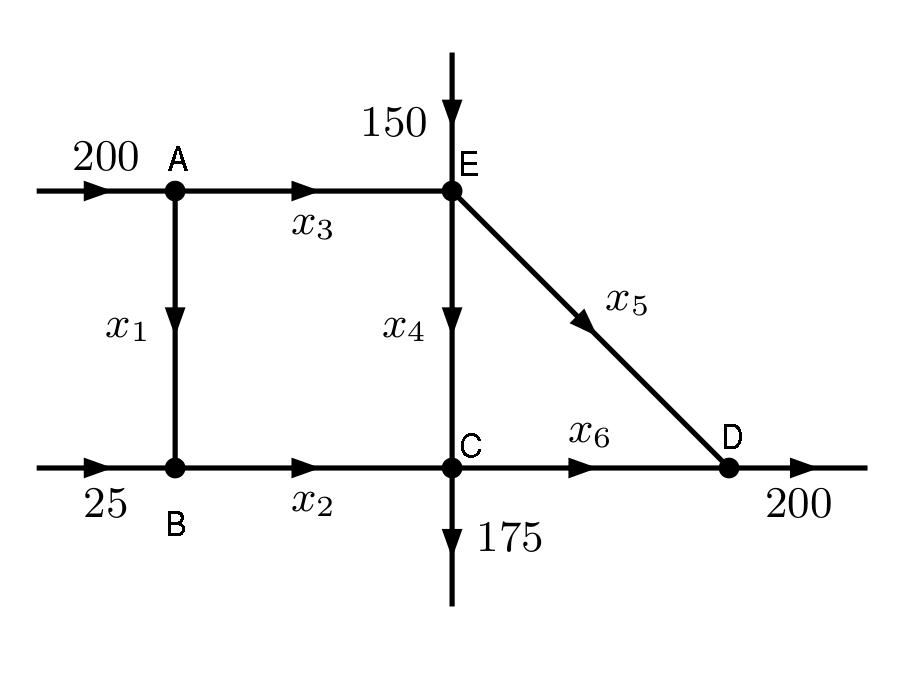
\includegraphics[scale=0.4]{q5.png}
\newpage
\subsection{a)}
The network equation and node equations are as follows:
\begin{align*}
\text{Network: }200+25+150-200-175&=0 \\
\text{Node A: }200-x_1-x_3&=0 \\
\text{Node B: }25+x_1-x_2&=0 \\
\text{Node C: }x_4+x_2-x_6-175&=0 \\
\text{Node D: }x_6+x_5-200&=0 \\
\text{Node E: }150+x_3-x_4-x_5&=0
\end{align*}
After a bit of rearranging we will get:
\begin{align}
\text{Network: }375&=375 \\
\text{Node A: }x_1+x_3&=200 \\
\text{Node B: }x_1-x_2&=-25 \\
\text{Node C: }x_2+x_4-x_6&=175 \\
\text{Node D: }x_5+x_6&=200 \\
\text{Node E: }x_3-x_4-x_5&=-150
\end{align}
Equation $(35)$ tells us that the amount of hydrocarbons flowing in equals to the amount flowing out.

\subsection{b)}
Putting equations from $(36)$ to $(40)$ into an augmented matrix we get:
\begin{align}
\left(\begin{array}{cccccc|c}
1 & 0 & 1 & 0 & 0 & 0 & 200 \\
1 & -1 & 0 & 0 & 0 & 0 & -25 \\
0 & 1 & 0 & 1 & 0 & -1 & 175 \\
0 & 0 & 0 & 0 & 1 & 1 & 200\\
0 & 0 & 1 & -1 & -1 & 0 & -150
\end{array}\right)
\end{align}
\newpage
Using GNU octave, the reduced echelon form of $(41)$ is:
\begin{align}
\left(\begin{array}{cccccc|c}
     1  &   0  &   0  &   1  &   0  &  -1 &  150 \\
     0  &   1  &   0  &   1  &   0  &  -1 &  175 \\ 
     0  &   0  &   1  &  -1  &   0  &   1 &  50 \\
     0  &   0  &   0  &   0  &   1  &   1 &  200 \\
     0  &   0  &   0  &   0  &   0  &   0 &  0 \\ 
\end{array}\right)
\end{align}
$x_1,x_2,x_3,x_5$ are leading variables and $x_4,x_6$ are free variables.
We let that $x_4 = s$ and $x_6 = t$.
\begin{align}
x_1+x_4-x_6&=150 \\
x_2+x_4-x_6&=175 \\
x_3-x_4+x_6&=50 \\
x_5+x_6&=200 \\
x_4&=s \\
x_6&=t
\end{align}
Solving each equation in turn gives:
\begin{align}
x_1&=150-s+t \\
x_2&=175-s+t \\
x_3&=50+s-t \\
x_5&=200-t \\
x_4&=s \\
x_6&=t
\end{align}
\subsection{c)}
If $x_4=50$ and $x_6 = 0$, We just throw the numbers back into Equation $(49)$ to $(54)$
\begin{align*}
x_1&=100 \\
x_2&=125 \\
x_3&=100 \\
x_5&=200 \\
x_4&=50 \\
x_6&=0
\end{align*}
\end{document}